%\documentclass[aps,prl,preprint,groupedaddress]{revtex4-1}
%\documentclass[aps,prl,preprint,superscriptaddress]{revtex4-1}
\documentclass[aps,prl,twocolumn,superscriptaddress]{revtex4-1}
%\documentclass[aps,pre,preprint,superscriptaddress]{revtex4-1}
%\documentclass[aps,pre,preprint,groupedaddress{revtex4-1}
\usepackage{graphicx}% Include figure files
\usepackage{dcolumn}% Align table columns on decimal point
\usepackage{bm}% bold math
\usepackage[centertags]{amsmath}
\usepackage{amsfonts}
\usepackage{amssymb}
\usepackage{amsthm}
\usepackage{newlfont}
\usepackage{color}
\usepackage{natbib}
\usepackage{subfigure}
 
\begin{document}

\title{Fast and Accurate Determination of Phase Transition Temperature in Computer Simulation}

\author{Mingzhe Shao}
\affiliation{Department of Packaging and Printing, Tianjin University of Science and Technology, Tianjin, China}

\author{Xin Zhou$^{*}$}
\affiliation{School of Physical Sciences, University of Chinese Academy of Sciences, Beijing 100049 China}

\date{\today}
 

\begin{abstract}  
Generalized canonical ensemble (GCE) simulations are performed in water/ice coexisting systems to obtain its phase transition temperature. For the first time, the equilibrium at water/ice coexisting state can be studied in an individual simulation. This equilibrium, no longer a stochastic process, leads to a remarkable increase in both efficiency and accuracy of determining melting points. In this study, TIP4P/2005, TIP4P/ICE, mW water model are applied to build Ice Ih/water two-phase systems, then equilibrated at distinct areas in energy surface. States such as bulk water, ice and water/ice coexisting have been evolved, and their corresponding temperature are gained at the same time. The result of phase transition temperature is in excellent agreement with previous studies, is 253K, 272K, and 274K, respectively. Results from small systems show subtle accuracy lost.  These features make GCE approach determining phase transition temperature robust, easy to use, and particularly good at working on computationally expensive systems.
\end{abstract}

\pacs{ } 

\maketitle{}
\section{Introduction}

The transition between different molecular structures induce significant changes in physical properties.  However, these changes are not yet well understood in many transitions, their mechanism at the molecular level remains largely unknown.
exp1:The transition between the ferromagnetic and paramagnetic phases of magnetic materials at the Curie point.
exp2:transition into superconductive state.
exp3: Hydrogen bonding between individual water molecules yields a disordered three-dimensional hydrogen-bond network whose rugged and complex global potential energy surface permits a large number of possible network configurations, ~\cite{Matsumoto2002} making water freezing one of the most intriguing phase transition system. 
These issues call forth more comprehensive knowledge of phase transition, especially the details in phases-coexisting systems(PCS). Studying PCS by performing direct canonical or isothermal–isobaric(NPT) ensemble is well performed worldwide and generally accepted, however the efficiency of this approach is largely determined by the nucleation energy barrier of PCS. Sampling critical states is hard since surface tension increased system energy leads to a less probability of being occupied. Besides, studying thermodynamics by sampling in non-equilibrium systems is controversial. 

Estimating transitional temperature is of absolute importance in describing PCS. The technique of direct coexistence is a first choice, studies have been carried out by simulating PCS in a temperature range, order parameters such as density are used to monitor the transition process. Transitional temperature is thus determined as the spinodal temperature of order parameter. However, evolution of states at critical temperature is stochastic, accuracy of this approach depends on not only sensitiveness of order parameter and the temperature interval in simulations, the sample volume matters as well. Another method is proposed by fitting the temperature dependence of free energy for both two phase, the intersection stands for the transitional temperature. This method shows better precision, but estimating free energy of systems is not convenient and takes extra work.

In this work, we aim to provide a simple method of high-precision and efficiency for determining the phase transition temperature in PCS. To achieve such goal, generalized canonical ensemble (GCE) has been implemented successfully in ice Ih/water PCS with mW, TIP4P-2005 and TIP4P-ICE water models. GCE can sufficiently visit the phase-coexistence regions and its energy distribution can be Gaussian-like. Thus the stochastic nature of phase transition can be largely get rid of, making one single simulation enough to estimate phase transition temperature. Besides the enhanced sampling in GCE expanded sample volume insure considerable precision of estimation.

This work is organized as follows: Sec. II describes the models and methodology used in this work. Section III presents the results for phase-coexistence region for different water potential models. The papers ends with a final discussion and the conclusions of this work.
\section{Models and Methods} 
\subsection{A. Water Models}
So far, water has been modeled in several different manner such as multi-site model\cite{Sanz2004,Bryk2002,Horn2005,Gonzalez2010,Kumar2012,Sedlmeier2011,Vega2007,Yu2013,Himoto2011}, implicit model\cite{Huißmann2012}, coarse-grained model\cite{Molinero2009,Marrink2004Coarse}. Multi-site mode have been widely applied to reveal the thermodynamic, dynamic, and structural anomalies of water\cite{Gao2000,Bryk2002,Sanz2004}, but some times computations can be very time-consuming, especially when it comes to water freezing at low supersaturation\cite{Mishima1998} . To observe puzzling behavior of water close and inside "no man's land"\cite{Moore2011}, a coarse-grained model mW water\cite{Molinero2009} using Stillinger-Weber (SW) potential to describe the tetrahedral hydrogen bond network in water and ice has been developed to accelerate the computation. In this paper, tip4p-2005, tip4p-ice and mW water models were applied to verify our method in determining phase transition temperature. In Table\ref{table:water model}  we present the geometry and the potential parameters of two popular potential full atom water models used in this work. 

\subsection{B. GCE/GNPT Method}

Generalized canonical ensemble(GCE)\cite{Xu2012} was first proposed to enhance sampling in systems with complex energy landscape. It is a direct generalization of canonical ensemble and can be regarded as a derivative of Hetherington's Gaussian ensemble.The conformational distribution $W_{gce}$ for GCE ensemble $f_{gce}{E}$ is

\begin{equation}
W_{gce}=exp[−f_{gce}(E)]\;,
\end{equation}

while $f_{gce}(E)$ is a particular function, or say, effective potential function in GCE, defined as
\begin{equation}
f_{gce}(E)=\beta E+ \frac{\alpha}{2}(E−U)^2\;.
\end{equation}
$\beta$, $\alpha$ and U are three parameters adjustable to control the energy distribution of system. $\beta$ is reversed temperature, U is a target energy value, and $\alpha$  is width factor of the energy distribution. It is an usual canonical ensemble if $\alpha=0$. The GCE ensemble can easily be obtained by setting the instant thermal coupling temperature as the first order derivative of ensemble function:
\begin{equation}
\widetilde{\beta}(E)≡\frac{f_{gce}(E)}{dE}≡\beta+\alpha(E−U)\;,
\end{equation}
To expand the universality of this method, a generalized isobaric-isothermal ensemble(GNPT) was developed in the same way, by defining ensemble function of entropy $H=E+PV$ rather than $E$:

\begin{equation}
f_{gce}(H)=\beta H+ \frac{\alpha}{2}(H−U)^2\;.
\end{equation}
and corresponding instant thermal coupling temperature as
\begin{equation}
\widetilde{\beta}(H)≡\frac{f_{gnpt}(H)}{dH}≡\beta+\alpha(H−U)\;,
\end{equation}

In a word,  GCE/GNPT can be applied to sufficiently visit the phase-coexistence regions, its energy distribution is Gaussian-like\cite{Xu2012,Xu2015}. And for the first time, this method is used to determine the phase transition temperature.

\subsection{C. Simulation Details}
In our work, system is built with 32480 or 4584 water molecules for mW (approximately $400 \AA \times 56 \AA \times 43 \AA$) and full atom water model (approximately $200 \AA \times 26 \AA \times 29 \AA$), respectively. Ice phase is extract from 20ns equilibrated bulk ice Ih at 260K, with x-y plane set as ice Ih basal plane, leaving the secondary prismatic plane ($1\overline{2}10$) in contact with bulk water. The two phases system are equilibrated for another 100 ps to produce the interfaces. The size in x direction is about 7 time of y and z direction, to ensure stable interfaces and study size effect in measuring phase transition temperature. Besides, systems of distinct size have been carried out to test the universality of this method.
All MD simulations were carried out in GNPT employing LAMMPS molecular dynamics code with GCE module\cite{Xu2012}. A Nosé−Hoover barostat\cite{Nose1984,Hoover1985} with  relaxation times 1 ps are used to keep the pressure fixed at 1atm. For full atom water model, a time step of 2\,fs  was used in all simulations. Lennard-Jones interactions are truncated smoothly at 14.0 Å. Nontruncated electrostatic interactions are treated by the particle-particle particle mesh solver (pppm) with a real space cutoff of 11.0 Å and precision tolerance of $10^{-5}$.  The mW water is built by following previous work of Molinero and co-workers\cite{Molinero2009} .
\section{Results and Discussion} 
The direct coexistence technique is to put in contact two or more phases in one simulation box and study its thermodynamics. This method is generally accepted in studying multi-phase systems and used very often in outlining phase diagram\cite{Conde2017,Sanz2004,Watanabe2012}. In our work, we still build our system in such classic way to clarify the effect induced by crystal lattice and interfacial crystal plane. And of course, save computational cost especially in freezing of full atom water. The coexisting system is balanced at 250K for 100 ps, this short simulation is not enough for system to attain equilibrium, but able to relax the interfaces and a energy value $H=E+PV$ can be extract to guide setting  energy value of GNPT simulations. For mw ice Ih/water case, this value is around $-10.7 kcal/mol$,  the GNPT equilibrated conformation with energy value range from $-9.1$ to $-11.3$ are shown in Fig\ref{fig:conformation}. The energy value can be simply regarded as the numerical average of water and ice energy, while lower value means more ice content. It is quite the same with unusal NPT ensemble if the equilibrated conformation is bulk phase, since energy distribution in bulk phase is always unimodal. That is, when H = -9.9,-10.1,-11.5 , GNPT ensembles act like NPT ensemble of bulk water at 312K,286K and bulk ice at 268K, as the evolutions of GNPT ensembles  shown in Fig.\ref{fig:evolution}.
\begin{figure}[ht]
\centering{}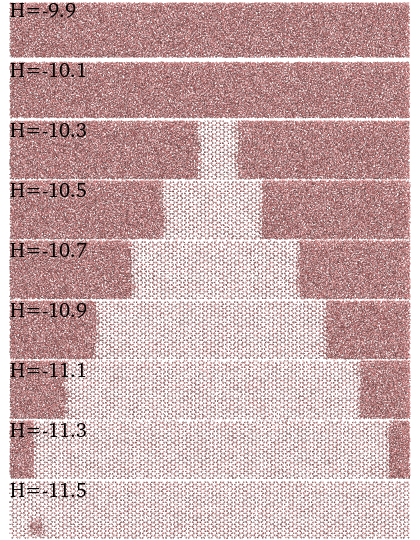
\includegraphics[width=0.5\textwidth]{conf.png} 
\caption{The conformations of GNPT ensembles at distinct energy levels: From bulk water above room temperature to completely freezed ice Ih.
\label{fig:conformation} }
\end{figure}

It takes a comparably short time (less than 2ns) for mW water to attain equilibrium. However, data between 5ns to 20ns are  sampled to generate its statistical average. Only former 5ns data is presented in Fig.\ref{fig:evolution} to focus on the equilibrating temperature uniformization (~275.1K) of evolutions in 2-phase coexisting systems. This uniformization is self-consistent, does not rely on initial setting, thus making this GCE/GNPT approach very adaptive. In Fig. \ref{fig:PTtemp-mw}, we compare the temperature of GNPT ensembles with referred melting point $274.6\pm 1$  \cite{Molinero2009} (color in cyan), the result shows good agreement. 
\begin{figure}[ht]
\centering{}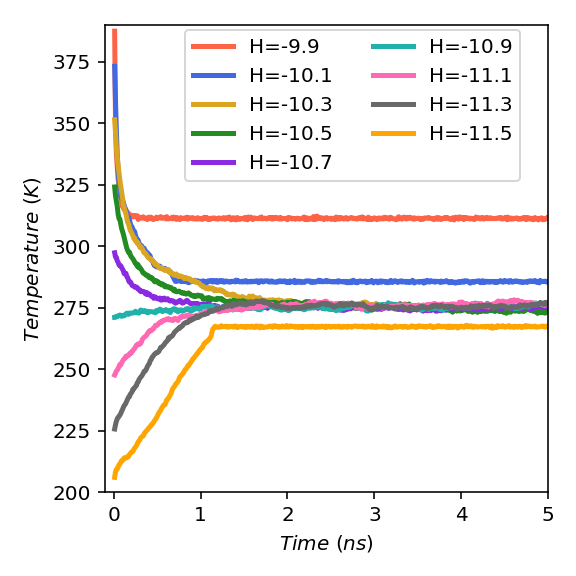
\includegraphics[width=0.5\textwidth]{PoteScan.png} 
\caption{The evolution of GNPT ensembles at distinct energy levels: Starting with a ice Ih/water coexisting state. Only the former 5ns equilibrium is plotted.
\label{fig:evolution} }
\end{figure}
It has to be point out, melting point we extract from GNPT ensembles of distinct energy level slightly differs. This reason is not yet clear, we ascribe thisas a size effect of ice phase for two reason. First, bulk ice are capable of adjusting their lattice to a lower energy level, leading a better thermostability, causing melting always happens on the interface rather than the bulk phase. Second, classic nucleation theory indicates that larger critical nuclei calls for a higher critical temperature.  We looking forward to a more comprehensive work to elucidate this effect. In this work, the transition temperature of ice Ih/water for mW water model $T_m=275.15K\pm 0.20K$ is determined as the uniformized value of phases coexisting GNPT ensembles. 

\begin{figure}[ht]
\centering{}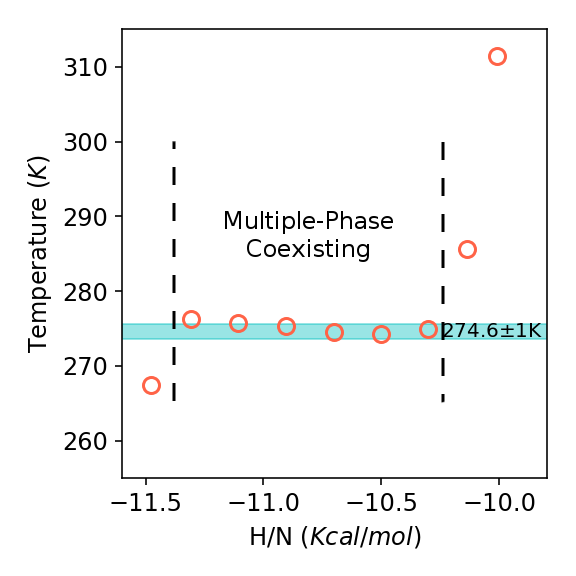
\includegraphics[width=0.5\textwidth]{PTtemp-mw.png} 
\caption{The phase transition temperature in GNPT ensembles. Dash line refers to 274.6K, the melting point for mW water proposed in previous study \cite{Molinero2009} . 
\label{fig:PTtemp-mw}} 
\end{figure}

To further explore the performance of this approach, we carried out more simulations of different system size. Three GNPT ensembles of 44800, 5971, 2030 water molecules are built  to apply the strategy, with size approximately $151\AA \times  156 \AA \times  58 \AA$, $54 \AA \times  58 \AA \times  58 \AA$, $52\AA \times  56 \AA \times  22\AA$ respectively.  Their result is colored in red in Fig. \ref{fig:sizeeffect},  which is $275.08\pm 0.17$, $275.00\pm 0.30$, and $275.21\pm 0.22$, while the black one is $275.08\pm 0.17$  from the uniformized value in Fig. \ref{fig:evolution}.

\begin{figure}[ht]
\centering{}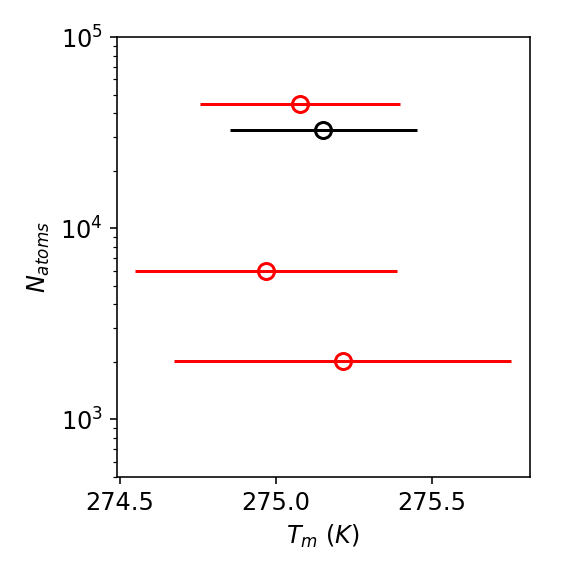
\includegraphics[width=0.5\textwidth]{size_effect.png} 
\caption{Size effect in GCE/GNPT method determined phase transition temperature. Data from Fig.\ref{fig:PTtemp-mw} is plot in black, the other data is extract from GNPT of 44800, 5971, 2030 water molecules, with size approximately $151\AA \times  156 \AA \times  58 \AA$, $54 \AA \times  58 \AA \times  58 \AA$, $52\AA \times  56 \AA \times  22\AA$,respectively.
\label{fig:sizeeffect}} 
\end{figure}
All these results match the refered $274.6\pm 1K$ , and even in the smallest system of 2030 molecules, its precision of melting temperature shows no obvious precision lost. This feature makes GCE/GNPT approach determining phase transition temperature of high precision, very fast and easy to use.

We further examine this approach by using full atom water model tip4p-2005 and tip4p-ice. The results is listed in Tab. \ref{table:PTtemp}, show excellent agreement with reference\cite{Abascal2005}.
 
 
 

%\section{Conclusions} 
As summary, we show that GCE/GNPT approach is very applicable of sampling metastable state, as we did in this work sampling phase transition state in water freezing. By following a classic 2-phase coexisting system direct simulation method, GCE/GNPT method is embeded to obtain its corresponding temperature for dinstinct energy levels. This temperature is the phase transition temperature if a intermediate state energy level is set. Precision of this approach is considerable and does not rely on system size. Results of mW, tip4p-2005, tip4p-ice water model show good agreements with references. This novel method is reliable, fast and easy to use.
    
%\section{Acknowledgement} 
The work is under the financial support of the NSFC Grant with No. 11574310, 11674345. C.-L. Wang thanks the support of the Youth Innovation Promotion Association, CAS. 

\section{Supplementary}

\begin{figure}[ht]
\centering{}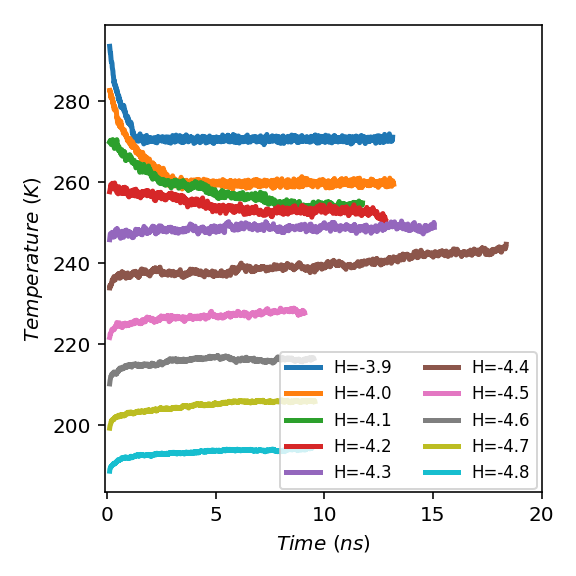
\includegraphics[width=0.5\textwidth]{PoteScan-2005.png} 
\caption{evolution of GNPT with tip4p-2005 water model
\label{fig:evolution-2005}} 
\end{figure}
\begin{figure}[ht]
\centering{}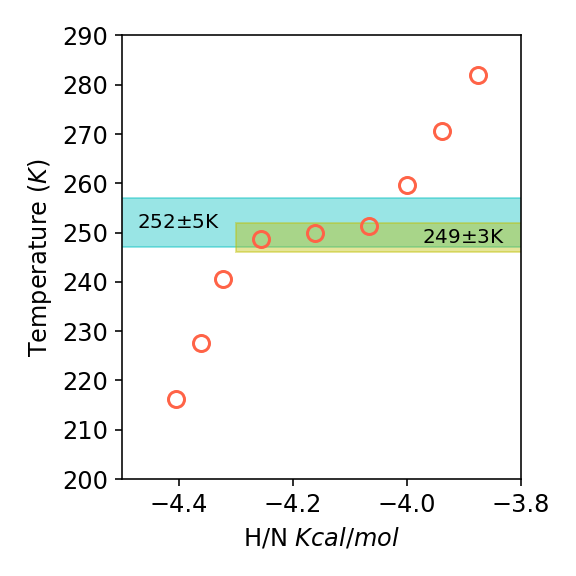
\includegraphics[width=0.5\textwidth]{PTtemp-2005.png} 
\caption{Phase transition temperature of GNPT with tip4p-2005 water model.
\label{fig:PTtemp-2005}} 
\end{figure}

\begin{figure}[ht]
\centering{}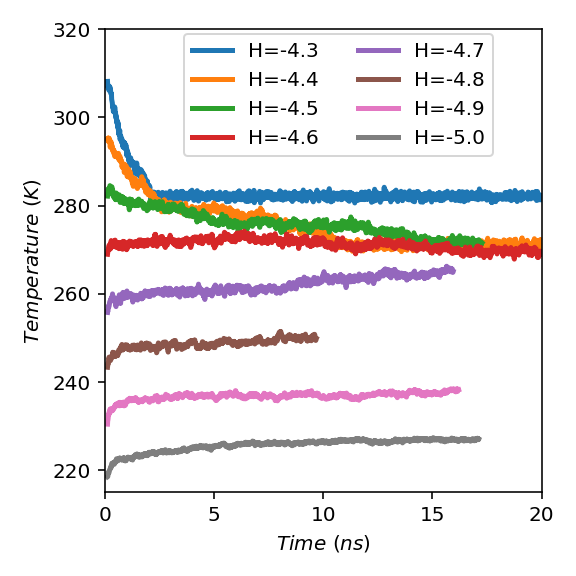
\includegraphics[width=0.5\textwidth]{PoteScan-ice.png} 
\caption{evolution of GNPT with tip4p-ice water model
\label{fig:evolution-ice}} 
\end{figure}
\begin{figure}[ht]
\centering{}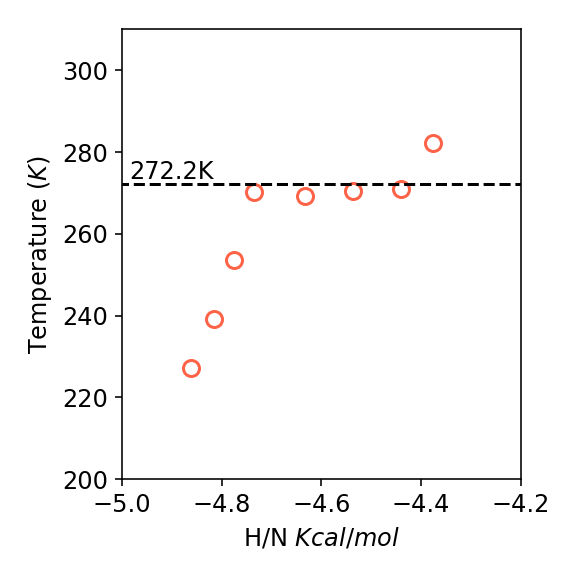
\includegraphics[width=0.5\textwidth]{PTtemp-ice.png} 
\caption{Phase transition temperature of GNPT with tip4p-icewater model.
\label{fig:PTtemp-ice}} 
\end{figure}




\begin{table}
\caption{Parameters of water model.}
\centering{}%
\begin{tabular}{ccccccc}
%\toprule 
\hline
{Model} & {$d_{oh}(\overset{\circ}{A})$} & { H-O-H}  & {$\sigma (\overset{\circ}{A})$}  & {$\epsilon/k (K)$} & {$q_H(e)$} 
\tabularnewline
%\midrule
\hline

{ TIP4P-2005} & { 0.9572} & {104.52}  & {3.3589}  & {93.20} & {0.5564}  \tabularnewline
{ TIP4P-ICE} & { 0.9572} & {104.52}  & {3.1668}  & {106.1} & {0.5897} \tabularnewline
%\bottomrule
\hline
\end{tabular}
\label{table:water model}
\end{table}


\begin{table}
\caption{Phase transition temperature of ice/water model.}
\centering{}%
\begin{tabular}{cccccc}
%\toprule 
\hline
{Model} & {TIP4P-2005} & {  TIP4P-ICE}  & {mW}  & {mW(ice Ic)}\tabularnewline
%\tabularnewline
%\midrule
\hline

{reference  $T_m (K)$} & {252.1} & {272.2}  & {274.6}  & {274.6} \tabularnewline
{This work} & { 252.1} & {272.2}  & {274.6}  & {274.6}\tabularnewline

%\bottomrule
\hline
\end{tabular}
\label{table:PTtemp}
\end{table}


%%%END OF MAIN TEXT%%%

\bibliography{gce-PTtemp}
%You need to replace "rsc" on this line with the name of your .bib file
%\bibliographystyle{rsc} %the RSC's .bst file

\end{document}